\subsection{Problem}

\renewcommand{\theequation}{\theenumi}
\begin{enumerate}[label=\thesection.\arabic*.,ref=\thesection.\theenumi]
\numberwithin{equation}{enumi}
	\item Find the angle between the x-axis and the line joining the points 
	\begin{align}
\vec{A} = \myvec{3\\-1}\text{ and }\vec{B} = \myvec{4\\-2}.
	\end{align}
	The following python code computes the angle which the line in Fig.\ref{fig:qnine} makes with x-axis.
	\begin{lstlisting}
	./codes/lines/q9.py
	\end{lstlisting}
	
	\solution Let the given line be represented as 
	\begin{align}
	\vec{u} = \vec{A-B} = \myvec{-1\\1}
	\end{align}
	x-axis can be represented as
	\begin{align}
	\vec{v} = \myvec{a\\0}
	\end{align}
where a$ \in \mathbb{R}$\\
\begin{align}
\vec{u}^T\vec{v} = \norm{\vec{u}}\norm{\vec{v}}\cos{\theta}
	\\
	\cos{\theta} = \frac{-a}{\sqrt{2}a}
	\\
	\cos{\theta} = \frac{-1}{\sqrt{2}}
	\\
	\theta = 135\degree 
\end{align}

	\begin{figure}[!ht]
	\centering
	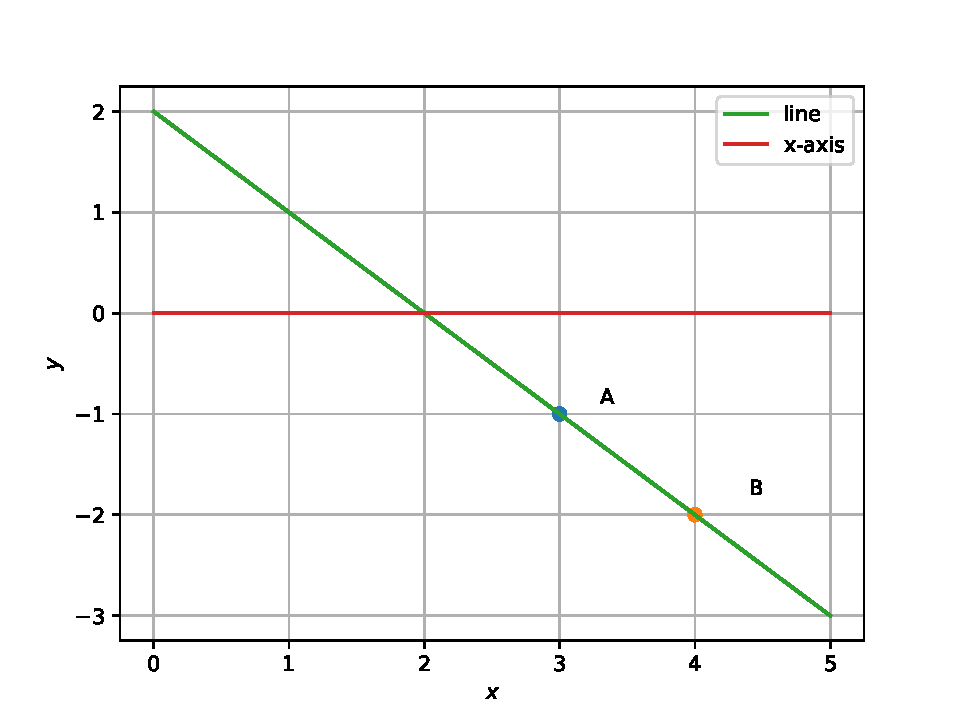
\includegraphics[width=\columnwidth]{./figs/lines/q9.pdf}
	\caption{Line of Q.3.5.5}
	\label{fig:qnine}	
	\end{figure}
	
\end{enumerate}

